

\documentclass[a4paper,12pt]{article}

\usepackage{times}
%\usepackage[margin=30mm]{geometry}
%% uncomment this to make the final no-margin layout
\usepackage[margin=8mm]{geometry}

\usepackage{pdfpages}

\usepackage{graphicx}
\usepackage{amssymb}
\usepackage{url}
\usepackage{amsmath,epsfig,graphics}
%\usepackage{natbib}
%\usepackage{wrapfig}
%\usepackage[rflt]{floatflt}
\usepackage[pdftex]{hyperref}
%\hypersetup{
%colorlinks,% 
%citecolor=black,% 
%filecolor=black,% 
%linkcolor=black,% 
%urlcolor=blue
%}

\newcommand{\eat}[1]{}
\newcommand{\TODO}[1]{ {\color{blue}{\bf TODO:~{#1}}} }
\newcommand{\bfheading}[1]{\noindent{\bf{#1}}}
\newcommand{\surl}[1]
{
	\urlstyle{same}\url{#1}
}

\pagestyle{empty}

\begin{document}

%Title         : GP-UCB for HMMs
%Author        : Lexing Xie
%Affiliation   : Australian National University
%Email         : lexing.xie@anu.edu.au
%
%Author        : Cheng Soon Ong
%Affiliation   : NICTA
%Email         : chengsoon.ong@anu.edu.au
%
%Colorizer     : javascript
%Bib style     : plainnat
%Bibliography  : example
%Heading base  : 2
%
%Doc class     : [11pt]article
%
%[TITLE]
%
%~ Abstract
%The abstract of the paper. Cum justo odio, dapibus ac facilisis in,
%egestas eget quam. Fusce dapibus, tellus ac cursus commodo, tortor
%mauris condimentum nibh, ut fermentum massa justo sit amet.
%~


\section{Introduction}

We consider two graphical models.

The first is a multiple output hidden Markov model (MOHMM) and is shown in Figure \ref{fig:mohmm}. 
This is also a convenient way to represent mixed output types, 
e.g. $p(a_t|z_t) \sim N(\mu_a, \sigma^2_a)$, 
$p(b_t|z_t) \sim \text{multinomial}(m_b)$.

%~ Figure { #fig-mohmm caption="multiple output hidden markov model" page-align=here }
%![gm-mohmm]
%~
\begin{figure}[!h]
\centering 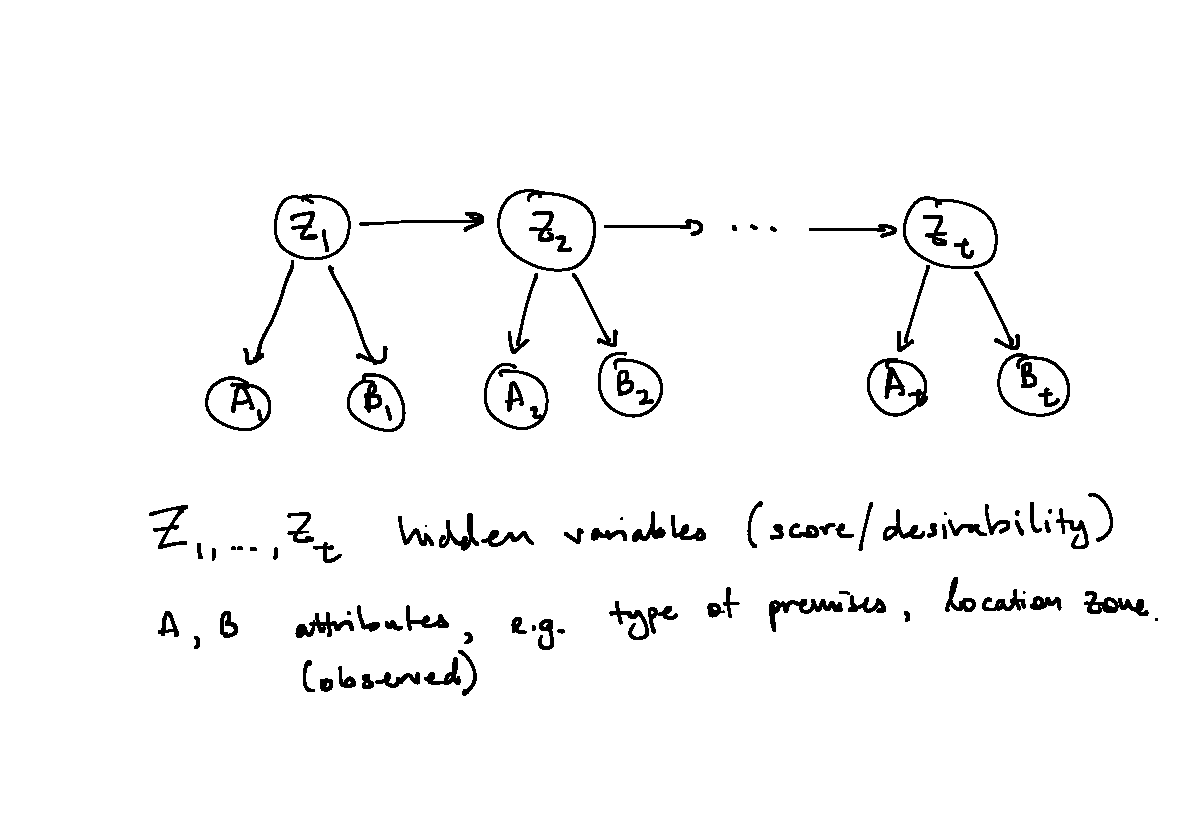
\includegraphics[width=0.75\textwidth]{figs/mohmm} 
\caption{multiple output hidden markov model. \label{fig:mohmm}}
\end{figure}


The second is a markov chain where at each time point, there is a diamond.
We refer to this as the diamond hidden markov model (DIAHMM) and it is shown in Figure \ref{fig:diahmm}.

%~ Figure { #fig-diahmm caption="diamond hidden markov model" page-align=here }
%![gm-diahmm]
%~
\begin{figure}[!h]
\centering 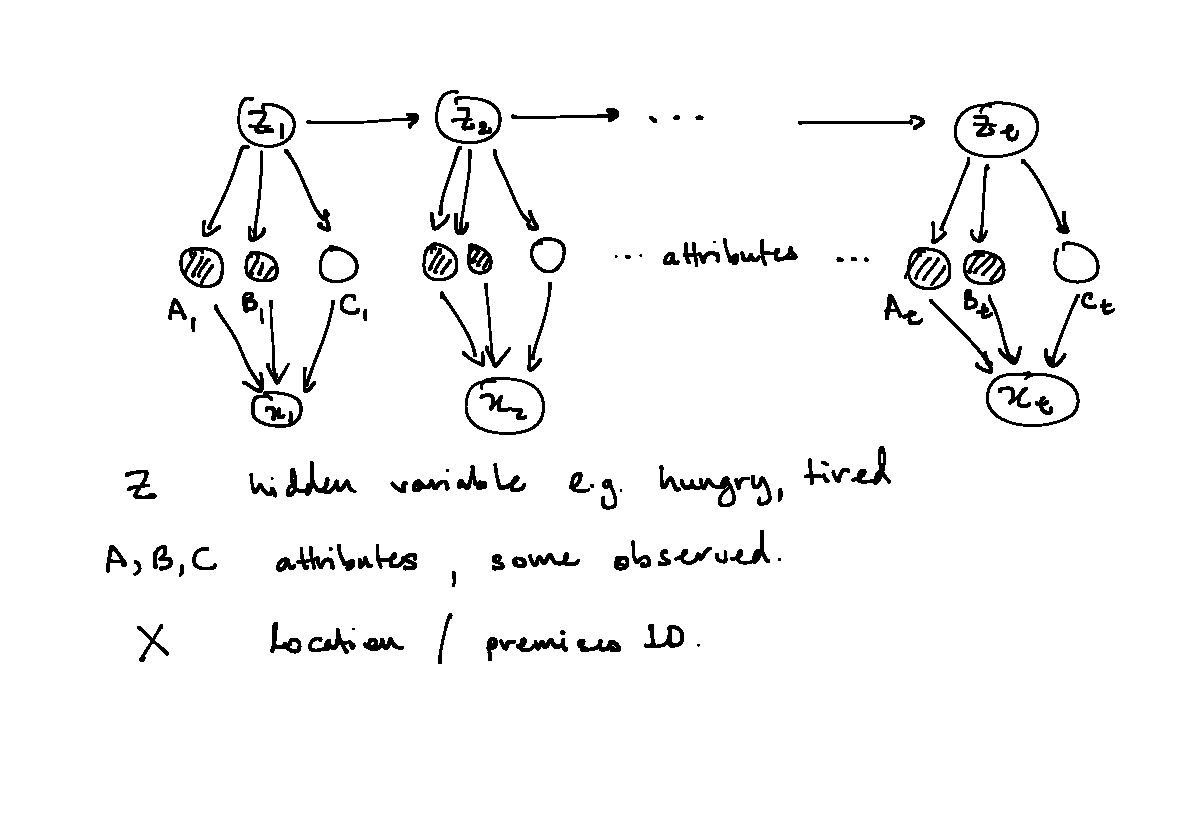
\includegraphics[width=0.75\textwidth]{figs/diahmm} 
\caption{diamond hidden markov model. \label{fig:diahmm}}
\end{figure}

%[gm-mohmm]: images/mohmm.png "mohmm"  { width=10 }
%[gm-diahmm]: images/diahmm.png "diahmm"  { width=10 }


\section{Bandit setting for (plain-vanilla) HMMs}

Assume there is a *prototypical* user $u$, whose behavior follows an HMM with parameter 
set $\Theta^*$. 

We don't know $\Theta^*$, therefore the system {\em guesses} a series of HMMs 
$\{ \Theta_t, t=1,2,\ldots T \}$, and uses them to (1) recommend actions $a_t$ to user $u$ and (2) observe rewards $r_t$ so as to update the current guess $\Theta_t$.  

A good strategy for generating action sequence $a_{1:T}$ and updating $\Theta_{1:T}$ needs to:

 Maximize {\em reward} e.g.
\begin{align}
  \max {\mathbb E} \sum_{t=1}^T r_t
\end{align} 
  OR *minimize regret*, make it as close to the *optimal* reward as possible
\begin{align}
  \min {\mathbb E}\sum_{t=1}^T r^*_t - {\mathbb E} \sum_{t=1}^T r_t
\end{align} 


Here defining *reward* is important, and *reward* does not seem *iid*. 

Given model $\Theta^*$, we can use the likelihood of 
the sequence $a_{1:t}$ as the *sum of the reward sequence*. 

\begin{align}
\sum_{1:t} r^*_t = P(a_{1:t} | \Theta^*) = \sum_{z_{1:t}} P(a_{1:t} | z_{1:t},  \Theta^*) 
\end{align} 

**Question** if we knew $\Theta^*$, can we generate one action sequence $a*_{1:t}$ such that the total reward is maximized? 
\begin{align}
{\mathbb R}^*_t = \max_{a_{1:t}} P(a_{1:t} | \Theta^*)
\end{align} 

%--------- 
%Our contributions are:
%
%* A figure of a _butterfly_;
%* Some **mathematics**;
%* And some source code;
%* And references to Tex books [@Knuth:tex;@Lamport:Latex;@Goo93;@FBerg04] and others [@Grandstrand]. 
%  Textual citations, like @Knuth:tex are also possible.
%
%# Content
%
%A definition of $e$ is shown in Equation [#euler] proved by Theorem [#th-euler]:
%
%~ Equation { #euler }
%e = \lim_{n\to\infty} \left( 1 + \frac{1}{n} \right)^n
%~
%
%~ Theorem {#th-euler}
%(_Euler's theorem_) More math here.
%~
%
%Let's program some Javascript:
%``` javascript
%function hello() {
%  return "hello world!"
%}
%```
%
%~ Note
%The syntax highlighting works in PDF too.
%~
%
%# Conclusion
%
%Really fun to write Markdown :-)

{
%\small
\bibliographystyle{abbrv}
\bibliography{BIB}
}

\end{document}

